%%*************************************************************************
%%
%% Anomaly detection by means of fourier tranform
%% V1.0
%% 2011/05/05
%% by Peter Boraros
%% See http://www.pborky.sk/contact for current contact information.
%%
%%*************************************************************************
%%
%% Legal Notice:
%%
%% This code is offered as-is without any warranty either expressed or
%% implied; without even the implied warranty of MERCHANTABILITY or
%% FITNESS FOR A PARTICULAR PURPOSE! 
%% User assumes all risk.
%%
%% This work by Peter Boraros is licensed under a 
%% Creative Commons Attribution-NonCommercial-ShareAlike 3.0 Unported License.
%% http://creativecommons.org/licenses/by-nc-sa/3.0/
%%
%%*************************************************************************

\documentclass[a4paper]{IEEEtran}

\usepackage{cite}
% \usepackage[nocompress]{cite}
\usepackage{ifpdf}

\ifpdf
\usepackage[pdftex]{graphicx}
\graphicspath{{./img/}}
\DeclareGraphicsExtensions{.pdf}
\else
\usepackage[dvips]{graphicx}
\graphicspath{{./img/}}
\DeclareGraphicsExtensions{.eps}
\fi

\usepackage[cmex10]{amsmath}
\usepackage{amsfonts}
\usepackage{amssymb}
\interdisplaylinepenalty=2500

\usepackage{algorithmic}

\usepackage{array}

\usepackage{mdwmath}
\usepackage{mdwtab}

\usepackage{eqparbox}

\usepackage[hang,small,center,bf]{caption}
% \usepackage[tight,normalsize,sf,SF]{subfigure}
%\usepackage[tight,footnotesize]{subfigure}
\usepackage{subfig}
% \usepackage[caption=false,font=normalsize,labelfont=sf,textfont=sf]{subfig}
% \usepackage[caption=false,font=footnotesize]{subfig}

\usepackage[utf8x]{inputenc}
\usepackage{url}
\usepackage{fixltx2e}
\usepackage{stfloats}
\usepackage{ucs}
\usepackage{multirow}

% correct bad hyphenation here
\hyphenation{op-tical net-works semi-conduc-tor}

\renewcommand{\labelitemi}{$\bullet$}
\renewcommand{\labelitemii}{$\circ$}
\renewcommand{\labelitemiii}{$\ast$}

\setlength{\textheight}{260mm}

\begin{document}
\title{Anomaly detection by means of fourier transform}
\date{July 7, 2011}
\author{Peter~Boraros %
\thanks{{Peter Boraros}, Czech technical university, Faculty of Electrical Engineering,
see~\texttt{http://www.pborky.sk/contact} for a contact infomation}}%

% The paper headers
\markboth{Peter Boraros, Czech technical university, Faculty of Electrical Engineering, Prague, Czech Republic}{}

\IEEEcompsoctitleabstractindextext{%
\begin{abstract}
The aim of this document is... 
\end{abstract}}

\maketitle
\IEEEdisplaynotcompsoctitleabstractindextext
\IEEEpeerreviewmaketitle

\section{Outline}
\[
IsHere(Succ(t),i) \Leftrightarrow
\forall x (\; (\underset{j \in Pr(i)}{\bigvee} (\; IsHere(t,i) \wedge CanPass(t,j,i) \;) \quad  ) \; \vee \; ( IsHere(t,i) \wedge \neg CanPass(t,i,x) ) \;)
\]

%\begin{figure*}[!h] %
%  \centering
%  \subfloat[PCA projection]{\label{fig:som_topol_proj_7}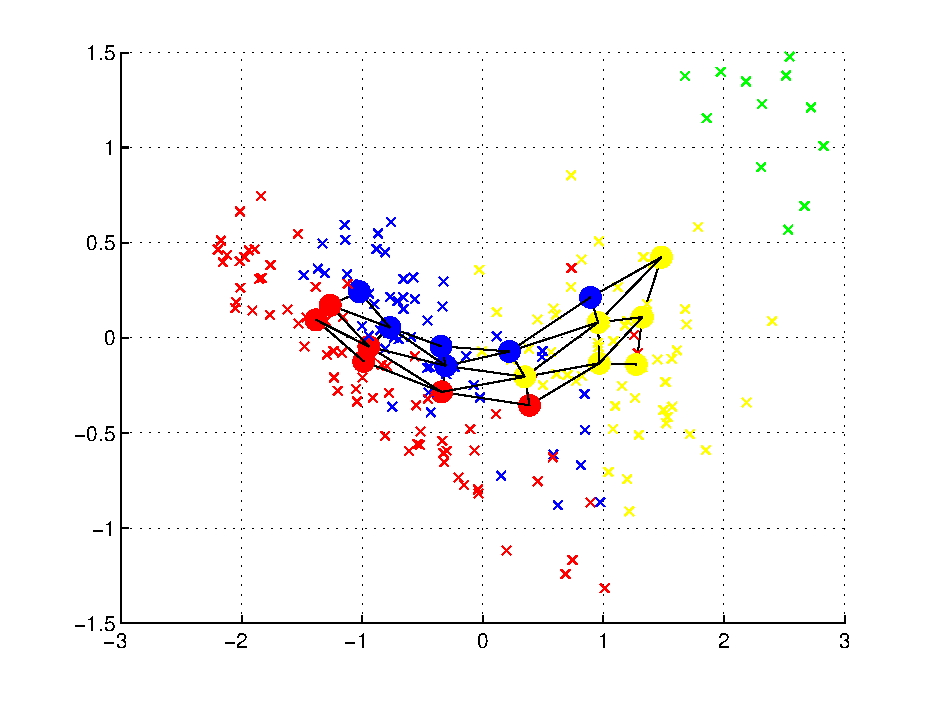
\includegraphics[width=55mm]{som_topol_proj_7}}
%  \subfloat[Sammon projection]{\label{fig:som_samon_proj_7}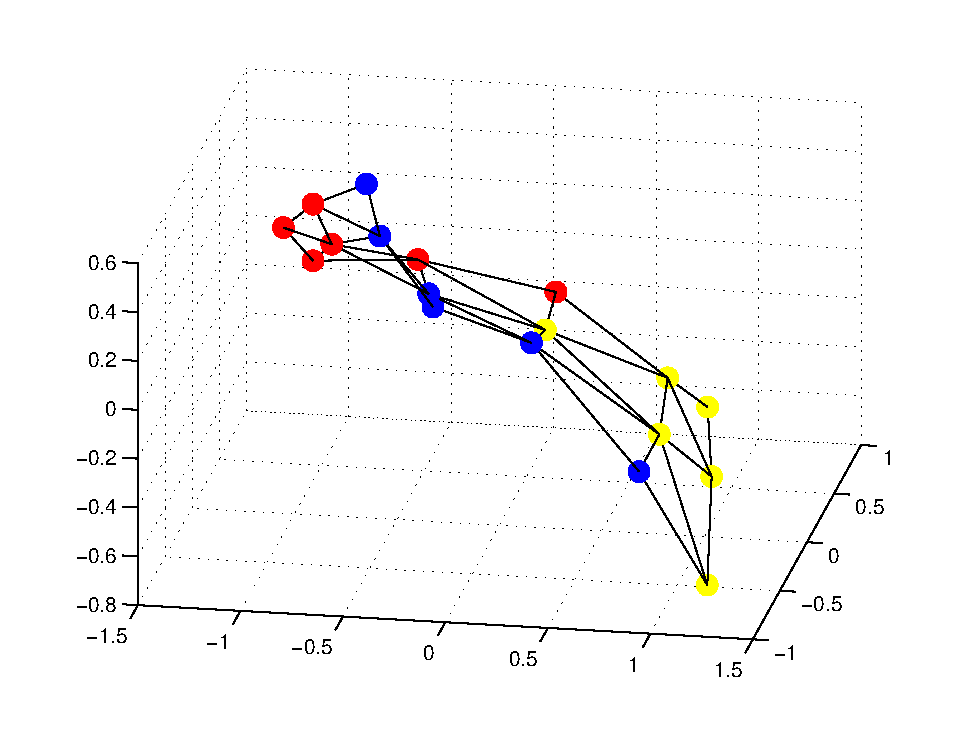
\includegraphics[width=55mm]{som_samon_proj_7}}
%  \subfloat[U-matrix and classification]{\label{fig:som_umat_7}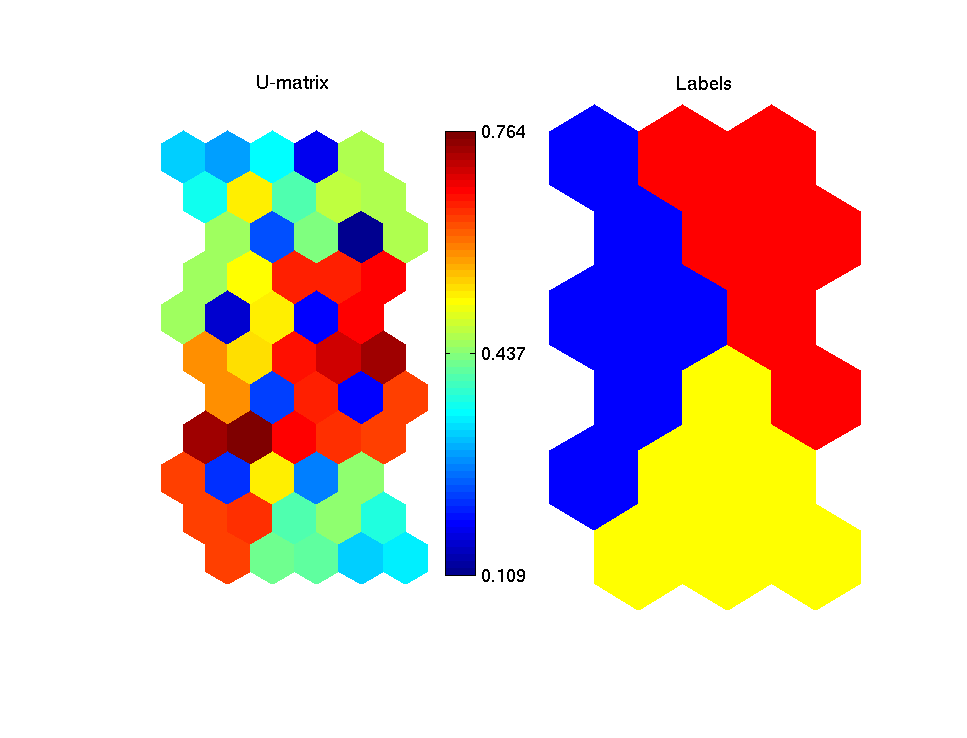
\includegraphics[width=55mm]{som_umat_7}}
%  \caption{configuration \#7 (see \textit{tbl. \ref{tbl:somresults}})}
%  \label{fig:som_config_7}
%\end{figure*}

% that's all folks
\end{document}
